\documentclass[preprint,12pt,a4]{standalone}
\usepackage{geometry}   % my added package "geometry"
\geometry{letterpaper,tmargin=1in,bmargin=1in,lmargin=2.5cm,rmargin=2.5cm}
\usepackage{tikz}
\usetikzlibrary{calc,patterns,arrows.meta,shapes.arrows,intersections,positioning}
\usetikzlibrary{decorations.pathmorphing,backgrounds,fit,petri}
\usepackage{standalone}
%
\begin{document}
	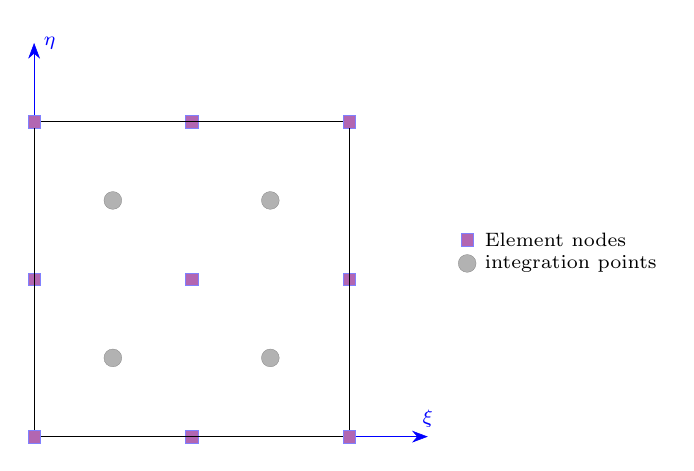
\begin{tikzpicture} [{place/.style={rectangle,draw=blue!50,fill=blue!20,ultra thin,inner sep=0.8mm}},{place2/.style={circle,draw=black!50,ultra thin,inner sep=0.8mm}},{linest/.style={color=gray,ultra thin}}]
		%axes
		\draw [{Stealth[length=2mm]}-{Stealth[length=2mm]}, help lines,blue] (5.0,0)node[above,font=\scriptsize]{$\xi$} -- (0.0,0.0) -- (0.0,5.0)node[right,font=\scriptsize] {$\eta$};
		%%element nodes
		\node at (0.0,0.0) [place,fill=violet!60] (1) {};
		\node at (4.0,0.0) [place,fill=violet!60] (2) {};
		\node at (4.0,4.0) [place,fill=violet!60] (3) {};
		\node at (0.0,4.0) [place,fill=violet!60] (4) {};
		\node at (2.0,0.0) [place,fill=violet!60] (5) {};
		\node at (4.0,2.0) [place,fill=violet!60] (6) {};
		\node at (2.0,4.0) [place,fill=violet!60] (7) {};
		\node at (0.0,2.0) [place,fill=violet!60] (8) {};
		\node at (2.0,2.0) [place,fill=violet!60] (9) {};
		
		%% integration points
	    \node at (1.0,1.0) [place2,fill=gray!60] (10) {};
		\node at (3.0,1.0) [place2,fill=gray!60] (11) {};
		\node at (1.0,3.0) [place2,fill=gray!60] (12) {};
		\node at (3.0,3.0) [place2,fill=gray!60] (13) {};
		%%element border
		\draw [-,black] (1) -- (2) -- (3) -- (4) --(1);
		%%middle nodes
		\node at (5.6,2.5) [right,font=\scriptsize]{$\mathrm{Element \ nodes}$};
		\node at (5.5,2.5) [place,fill=violet!60] (4) {};
		\node at (5.6,2.2) [right,font=\scriptsize]{$\mathrm{integration \ points}$};
		\node at (5.5,2.2) [place2,fill=gray!60] (4) {};
		
	\end{tikzpicture}
\end{document}